\chapter{Proposed Methodology}
\sloppy

\section{Overview}

\textbf{Goal.} ChromaGuide is a three-component framework for \sgRNA\ design that couples (i) \textbf{on-target efficacy prediction}, (ii) \textbf{off-target prediction} (unintended cleavage-site risk), and (iii) an \textbf{integrated \sgRNA\ design score} that balances predicted efficiency and specificity.

\textbf{Task 1 (on-target).} Given a guide/target pair in a cellular context, predict on-target efficacy $y\in[0,1]$ and (optionally) output a prediction interval with target coverage $1-\alpha$.

\textbf{Task 2 (off-target).} Given a candidate \sgRNA\ and a reference genome, identify plausible unintended cleavage sites and score their cleavage likelihood/severity, producing an aggregated off-target risk summary.

\textbf{Task 3 (design score).} Combine the calibrated on-target signal with the aggregated off-target risk to produce an overall \sgRNA\ design score for ranking candidate guides.

\textbf{Inputs.}
\begin{itemize}
\item \textbf{Sequence} $x_s$: \sgRNA\ protospacer+\PAM{} and target-site sequence context.
\item \textbf{Epigenomics} $x_e$: accessibility/histone-mark tracks summarized in a fixed window around (on-target and, when available, off-target) cut sites.
\item \textbf{Genome index/search} $\mathcal{G}$: reference genome data structure used to enumerate candidate off-target loci.
\end{itemize}

\textbf{Core modules (baseline design; subject to empirical validation).}
\begin{itemize}
\item On-target encoders: sequence encoder $z_s=g_s(x_s)$ and epigenomic encoder $z_e=g_e(x_e)$.
\item On-target fusion: $z=f([z_s;z_e])$ (baseline concatenation; optional attention/gating; optional non-redundancy regularizer).
\item On-target head: bounded-outcome head producing $(\mu,\phi)$ (baseline Beta regression) and conformal prediction for calibrated intervals~\citep{vovk2005,romano2019,barber2023}.
\item Off-target candidate generation: enumerate candidate loci using genome-wide approximate matching (PAM-constrained) with a bounded mismatch/bulge policy.
\item Off-target scoring network: score each candidate off-target site using sequence mismatch features and optional local context features (sequence, chromatin accessibility when available).
\item Design-score aggregator: combine the on-target prediction with an aggregated off-target risk to produce a single \sgRNA\ design score.
\end{itemize}


\begin{figure}[htbp]
\centering
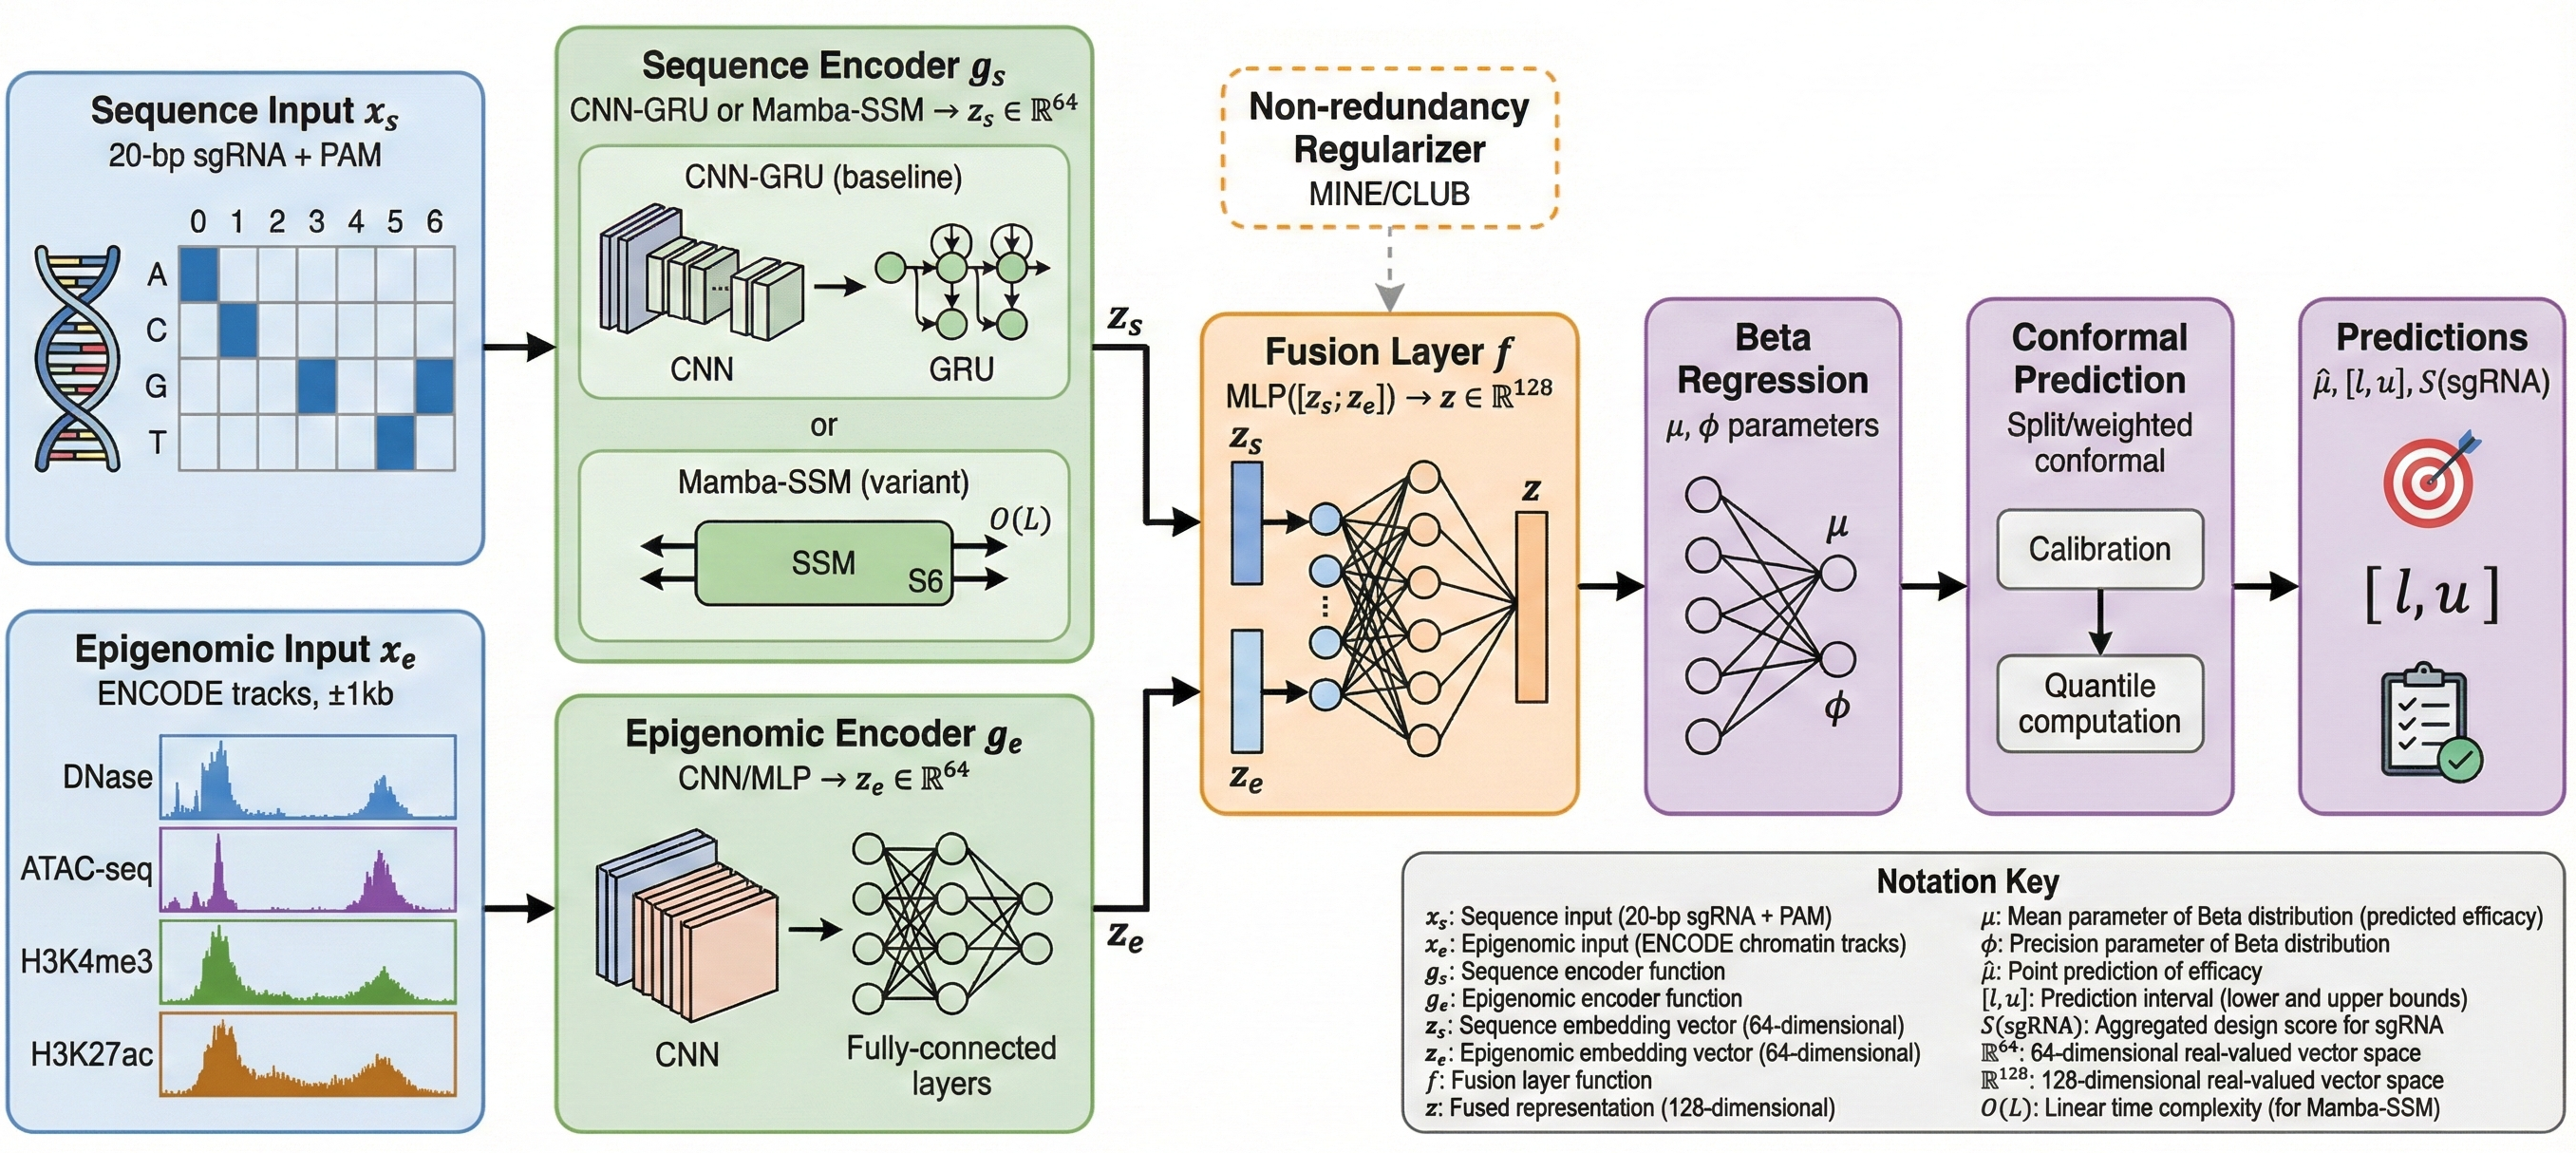
\includegraphics[width=\textwidth]{Figs/ChromaGuide.png}
\caption{\sloppy ChromaGuide architecture overview. The framework fuses sequence representations with epigenomic context features through a fusion layer. The sequence encoder supports two architectures: (1) a CNN-GRU baseline, or (2) a Mamba-based state-space model (SSM) variant with bi-directional processing and $O(L)$ linear complexity. Inputs: $\mathbf{x}_s$ (one-hot encoded 23-nt sgRNA+PAM sequence (20-nt protospacer + 3-nt PAM)), $\mathbf{x}_e$ (epigenomic tracks). Encoders: $g_s$ (sequence encoder) and $g_e$ (epigenomic encoder) produce embeddings $\mathbf{z}_s, \mathbf{z}_e \in \mathbb{R}^{64}$. Fusion layer $f$ produces $\mathbf{z} \in \mathbb{R}^{128}$. Beta regression outputs parameters $\mu$ (mean) and $\phi$ (precision). Conformal prediction generates calibrated intervals. Final outputs: point prediction $\hat{\mu}$, prediction interval $[l, u]$, and design score $S(\text{sgRNA})$. Optional non-redundancy regularizer (MINE/CLUB) encourages complementary representations.}
\label{fig:proposed-architecture}
\end{figure}

\section{Model architecture}


\subsection{\texorpdfstring{Sequence encoder $g_s$}{Sequence encoder gs}}

\begin{sloppypar}
Baseline: ChromeCRISPR-style CNN--GRU on 23-nt sgRNA+\PAM{} (CNN kernels 3/5/7 $\to$ BiGRU hidden 128 $\to$ pooled $z_s\in\mathbb{R}^{128}$). As contemporary alternatives, we will evaluate (i) hybrid architectures with dynamic feature weighting as in CRISPR\_HNN~\citep{li2025crisprhnn} and (ii) pretrained language-model embeddings for cross-variant generalization as in PLM-CRISPR~\citep{hou2025plmcrispr}. Transformer-based DNA/RNA embeddings are treated as optional extensions and ablated.
\end{sloppypar}

\begin{sloppypar}
Beyond Transformers, we will explore \textbf{state-space models (SSMs)} as an alternative sequence encoder architecture. Mamba~\cite{gu2023mamba} introduced selective state spaces with input-dependent gating, achieving linear-time complexity $O(L)$ while maintaining expressive long-range modeling. For genomic applications, Caduceus~\cite{schiff2024caduceus} extended Mamba with bi-directional processing and reverse-complement (RC) equivariance, demonstrating superior performance on long-range DNA sequence tasks at the ICML 2024 conference. The Evo model~\cite{nguyen2024evo} scaled long-context genome modeling to 131kb using the StripedHyena architecture (a hybrid attention + long convolution design), demonstrating that long-range encoders can capture regulatory elements across large genomic loci. Recent work on DNABERT-Epi~\cite{kimata2025dnabertepi} demonstrated that integrating epigenetic features with pre-trained DNA language models significantly improves CRISPR off-target prediction. We will benchmark a Mamba-based variant of our sequence encoder against the CNN-GRU baseline, evaluating whether SSMs provide computational efficiency gains without sacrificing predictive accuracy for sgRNA design tasks.
\end{sloppypar}


\subsection{\texorpdfstring{Epigenomic encoder $g_e$}{Epigenomic encoder ge}}

For each assay (e.g., DNase/ATAC, H3K4me3, H3K27ac), extract a window (default $\pm 1$ kb) around the cut site, bin into fixed-length features, apply log1p and training-only standardization, and map through an MLP to $z_e\in\mathbb{R}^{64}$. Additional tracks/encoders (e.g., 1D CNNs over binned tracks) may be used if empirically justified.

\subsection{\texorpdfstring{Fusion $f$ and optional non-redundancy regularizer}{Fusion f and optional non-redundancy regularizer}}

Baseline fusion is concatenation + MLP: $z=\mathrm{MLP}([z_s;z_e])\in\mathbb{R}^{128}$. If needed, replace with gating/cross-attention/mixture-of-experts.

We optionally encourage complementary representations with an information-theoretic objective:
\begin{equation}\label{eq:fusion}
f^* = \arg\max_{f \in \mathcal{F}} \left[ I(f(X_s, X_e); Y) - \lambda \cdot I(X_s; X_e | Y) \right],
\end{equation}
implemented with neural MI estimators (e.g., MINE/CLUB)~\citep{belghazi2018,cheng2020} and treated strictly as an ablation.

\subsection{Prediction head (Beta regression)}

Predict a Beta mean and precision:
\begin{equation}
\mu = \sigma(W_\mu z + b_\mu),\qquad \phi = \exp(W_\phi z + b_\phi).
\end{equation}
Negative log-likelihood:
\begin{equation}\label{eq:beta_loss}
\begin{split}
L = -\sum_{i=1}^N \Big[ &\log \Gamma(\phi_i) - \log \Gamma(\mu_i \phi_i) - \log \Gamma((1-\mu_i)\phi_i) \\
&\quad + (\mu_i \phi_i - 1) \log y_i + ((1-\mu_i)\phi_i - 1) \log(1-y_i) \Big].
\end{split}
\end{equation}
We clip $y$ to $(\varepsilon,1-\varepsilon)$ when needed; Beta regression is standard for continuous outcomes in $(0,1)$~\citep{ferrari2004beta}.

\section{Uncertainty quantification via conformal prediction}

Split conformal prediction yields distribution-free prediction intervals \emph{under the exchangeability assumption}~\citep{vovk2005,romano2019}. With a Beta head, define
$$
\hat{\sigma}=\sqrt{\frac{\hat{\mu}(1-\hat{\mu})}{1+\hat{\phi}}},\qquad s=\frac{|y-\hat{\mu}|}{\hat{\sigma}+\varepsilon}.
$$
On calibration data compute $\hat{\eta}=\mathrm{Quantile}_{1-\alpha}(\{s_i\})$ and output
$$
C(x)=\left[\hat{\mu}(x)-\hat{\eta}\,\hat{\sigma}(x),\;\hat{\mu}(x)+\hat{\eta}\,\hat{\sigma}(x)\right]\cap[0,1].
$$
For dataset/cell-line shift (Splits B/C), use weighted conformal calibration, which relies on (estimated) importance weights / likelihood ratios and may degrade under severe shift~\citep{barber2023}.

\section{Off-target prediction module}

\subsection{Candidate unintended-site identification}

Given a candidate \sgRNA\, ChromaGuide first enumerates plausible off-target loci by scanning the reference genome for PAM-adjacent protospacer matches under an explicit mismatch/bulge policy. Concretely, we (i) require a valid PAM (e.g., NGG for SpCas9; optionally extend to alternative PAMs when modeling SpCas9 variants), (ii) allow up to $k$ mismatches with position-dependent weighting (penalizing mismatches less in distal regions than in the seed), and (iii) optionally allow a small number of DNA/RNA bulges, depending on computational feasibility.

This stage outputs a set of candidate off-target sites $\{o_j\}$, each with its genomic coordinates and an alignment summary (mismatch positions/types and bulge indicators). To keep the proposal implementable and the document within a $\sim$30-page scope, we treat the genome search as a modular component (e.g., using an indexed approximate matching routine) and focus the research contribution on learning to score the resulting candidate set.

\subsection{Off-target scoring}

For each candidate site $o_j$, we compute a feature vector that includes (a) aligned guide--DNA sequence pairs / mismatch pattern encodings, (b) local sequence context around the cut site, and (c) optional cell-context features (e.g., accessibility) when tracks are available for the corresponding locus. This is motivated by recent off-target models that integrate epigenetic tracks with sequence representations (e.g., DNABERT-Epi)~\citep{kimata2025dnabertepi}. A neural scoring function outputs a per-site risk $r_j\in[0,1]$ that is intended to correlate with cleavage likelihood and/or editing readouts in available off-target datasets.

To summarize genome-wide risk for a guide, we aggregate across sites using a soft-max/Noisy-OR style pooling function, for example
$$
R(\sgRNA)=1-\prod_j (1-r_j) \quad \text{or} \quad R(\sgRNA)=\sum_j w_j r_j,
$$
where weights $w_j$ can encode distance-to-gene, exonic overlap, or other application-driven severity terms. As an additional baseline family for off-target scoring, we will consider language-model-based off-target predictors such as CCLMoff~\citep{du2025cclmoff}.

\section{Integrated \sgRNA\ design score}

ChromaGuide ranks candidate guides using an integrated design score that explicitly trades off efficiency and specificity. This is aligned with recent \sgRNA\ prediction/design models that explicitly integrate richer guide representations (e.g., sequence + secondary structure via graph neural networks in Graph-CRISPR)~\citep{jiang2025graph-crispr}. Let $\hat{\mu}(\sgRNA)$ denote the predicted on-target efficacy (mean of the bounded head) and let $R(\sgRNA)$ denote aggregated off-target risk. A simple, interpretable baseline is
$$
S(\sgRNA)=\hat{\mu}(\sgRNA)-\lambda\,R(\sgRNA),
$$
with $\lambda>0$ controlling the efficiency--specificity trade-off; alternative monotone combinations (e.g., $S=\hat{\mu}\cdot(1-R)$) are treated as ablations.

When uncertainty estimates are available, we will also evaluate risk-aware ranking rules that down-weight uncertain high-efficacy predictions (e.g., replacing $\hat{\mu}$ with a lower confidence bound).

\section{\sgRNA\ design tool / interface module}\label{sec:design-interface}

To satisfy the third ChromaGuide module requirement (a user-facing design capability rather than only predictive models), we will implement an interface that accepts either (i) a genomic target region (e.g., gene name / coordinates) or (ii) a user-provided DNA sequence, enumerates candidate protospacers with valid PAMs, and returns a ranked list with supporting diagnostics. This is conceptually similar to widely used \sgRNA\ design tools (e.g., CRISPOR and CHOPCHOP) but adds uncertainty-aware on-target estimates and an explicit chromatin-aware risk model~\citep{haeussler2016,labun2016chopchop}.

\paragraph{Inputs.} User-selected genome build; target coordinates or sequence; nuclease/PAM (SpCas9 NGG by default); optional cell type / epigenomic context (select ENCODE track set or upload summarized tracks).

\paragraph{Outputs.} For each candidate guide: predicted on-target efficacy (with interval), aggregated off-target risk $R(\sgRNA)$, integrated design score $S(\sgRNA)$, and a short explanation panel (top contributing sequence positions and key epigenomic bins). The tool will also export results as a CSV/TSV report to support downstream wet-lab planning.

\paragraph{Workflow (high level).}
\begin{enumerate}
\item Enumerate candidate guides in the target region under PAM and basic filters (e.g., homopolymer and GC constraints).
\item Compute on-target predictions with epigenomic integration when context is available; otherwise fall back to sequence-only mode.
\item Enumerate and score candidate off-target loci genome-wide, aggregate $R(\sgRNA)$, and compute $S(\sgRNA)$.
\item Rank guides and present the top-$K$ candidates with uncertainty-aware summaries.
\end{enumerate}

\section{Practical considerations (brief)}

\textbf{Missing epigenomics (modality dropout training).} Train with modality dropout by masking $x_e$ (or assay subsets) with probability $p$ and adding a missingness indicator, so the model degrades to sequence-only behavior when tracks are absent.

\textbf{Optional extensions.} RNA-FM embeddings, a lightweight \gRNA\ structure branch, and transfer initialization (PRIDICT/PrimeNet, or comparable alternatives) are optional and always ablated.

\textbf{Implementation defaults.} Adam/AdamW~\citep{kingma2015,loshchilov2019}, early stopping on calibration, and tuning restricted to train+calibration splits.

\section{Evaluation plan (summary)}

\textbf{Datasets.} Primary (initial): DeepHF~\citep{wang2019}. Stress tests (initial): CRISPRon~\citep{xiang2021} and CRISPR-FMC~\citep{li2025crisprfmc}.

\textbf{Splits (leakage-controlled).}
\begin{itemize}
\item \textbf{Split A (primary):} gene-held-out split on DeepHF with train/cal/test by gene.
\item \textbf{Split B (stress test):} dataset-held-out evaluation (e.g., leave-one-dataset-out across CRISPR-FMC constituents).
\item \textbf{Split C (stress test):} cell-line-held-out evaluation (train excluding one cell line; test on held-out line).
\end{itemize}

\begin{figure}[htbp]
\centering
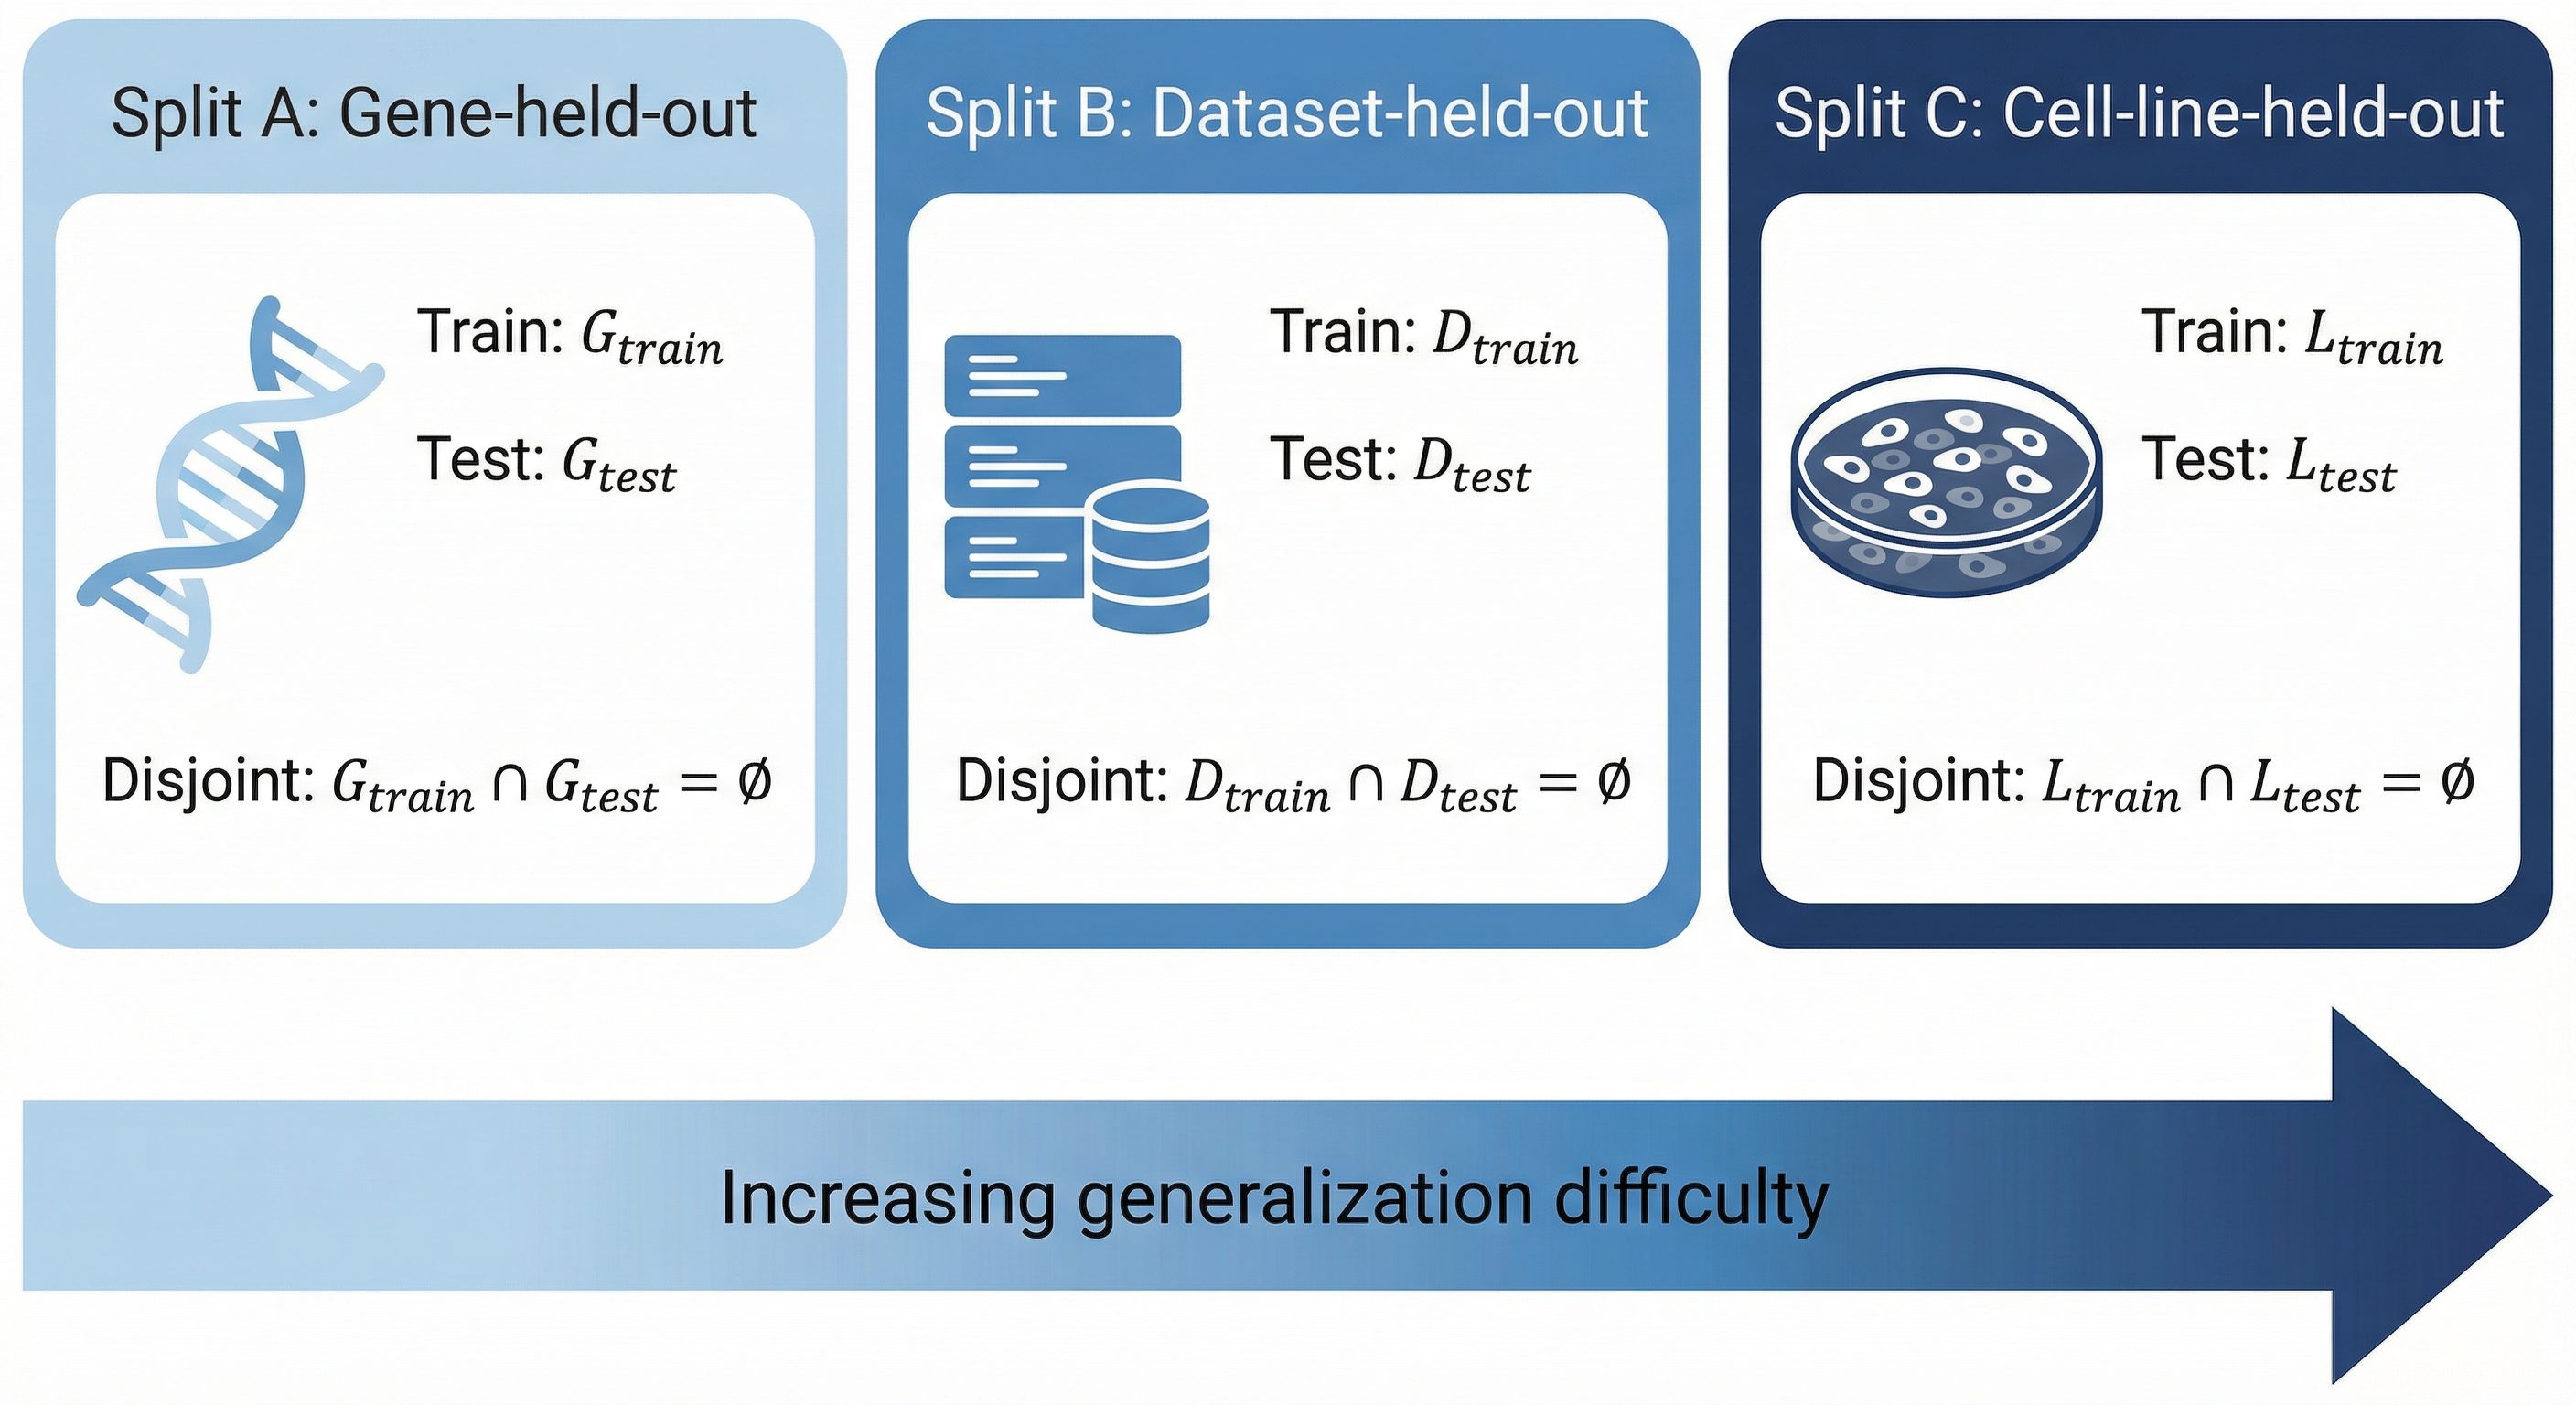
\includegraphics[width=\textwidth]{Figs/Data.png}
\caption{Evaluation protocol with three split types: (A) gene-held-out generalization, (B) dataset-held-out transfer across screen collections, and (C) cell-line-held-out deployment shift.}
\label{fig:eval-protocol-splits}
\end{figure}

We remove exact duplicate sequences globally; optionally repeat Split A under a conservative similarity filter as a sensitivity analysis.

\begin{sloppypar}
\textbf{Baselines.} ChromeCRISPR (sequence+GC)~\citep{daneshpajouh2025chromecrispr} and DeepHF~\citep{wang2019}; include CRISPRon~\citep{xiang2021} where comparable inputs are available. We additionally follow the ChromeCRISPR benchmark protocol for model comparison and reporting~\citep{daneshpajouh2025chromecrispr}. All models are evaluated on identical splits and preprocessing.
\end{sloppypar}

\textbf{Metrics.} Primary: Spearman correlation. Uncertainty: empirical coverage, mean interval width, and coverage stratified by dataset/cell line.

\textbf{Statistical reporting.} Report gene-level bootstrap confidence intervals for Spearman on Split A; use paired, gene-level permutation tests for model comparisons (with FDR control when many ablations are tested).

\begin{sloppypar}
\textbf{Ablations.} Leave-one-component-out on Split A: remove epigenomics; replace fusion objective with simple concatenation; remove optional embeddings/structure/transfer; compare unweighted vs. weighted conformal.
\end{sloppypar}

\section{Interpretability and attribution analysis}\label{sec:interpretability}

We use lightweight attribution analyses to connect predictions to biologically meaningful features.

\paragraph{Sequence-level attribution.}
Compute nucleotide-level saliency (e.g., integrated gradients) over the protospacer+\PAM{}.

\paragraph{Context-level attribution.}
Quantify which epigenomic assays/bins most influence predictions (e.g., attention/gating weights when available, or SHAP on summarized features) and report aggregated patterns across Split A and the held-out domains in Splits B/C.
